% !TEX TS-program = pdflatex
% !TEX encoding = UTF-8 Unicode

% This is a simple template for a LaTeX document using the "article" class.
% See "book", "report", "letter" for other types of document.

\documentclass[11pt]{article} % use larger type; default would be 10pt

\usepackage[utf8]{inputenc} % set input encoding (not needed with XeLaTeX)

%%% Examples of Article customizations
% These packages are optional, depending whether you want the features they provide.
% See the LaTeX Companion or other references for full information.

%%% PAGE DIMENSIONS
\usepackage{geometry} % to change the page dimensions
\geometry{a4paper} % or letterpaper (US) or a5paper or....
\geometry{margin=1in} % for example, change the margins to 2 inches all round
% \geometry{landscape} % set up the page for landscape
%   read geometry.pdf for detailed page layout information

\usepackage{graphicx} % support the \includegraphics command and options

% \usepackage[parfill]{parskip} % Activate to begin paragraphs with an empty line rather than an indent

%%% PACKAGES
\usepackage{booktabs} % for much better looking tables
\usepackage{array} % for better arrays (eg matrices) in maths
\usepackage{paralist} % very flexible & customisable lists (eg. enumerate/itemize, etc.)
\usepackage{verbatim} % adds environment for commenting out blocks of text & for better verbatim
\usepackage{subfig} % make it possible to include more than one captioned figure/table in a single float
% These packages are all incorporated in the memoir class to one degree or another...
\usepackage{enumitem}
\usepackage{amsmath}

% para los cuadritos en links
%\usepackage[linkbordercolor={0 0 1}, citebordercolor={0 1 0}, urlbordercolor={1 0 0}]{hyperref}
\usepackage[colorlinks=true, linkcolor=black, citecolor=green, urlcolor=red]{hyperref} % solo resalta
\usepackage[spanish]{babel}



%%% HEADERS & FOOTERS
\usepackage{fancyhdr} % This should be set AFTER setting up the page geometry
\pagestyle{fancy} % options: empty , plain , fancy
\renewcommand{\headrulewidth}{0pt} % customise the layout...
\lhead{}\chead{}\rhead{}
\lfoot{}\cfoot{\thepage}\rfoot{}

%%% SECTION TITLE APPEARANCE
\usepackage{sectsty}
\allsectionsfont{\sffamily\mdseries\upshape} % (See the fntguide.pdf for font help)
% (This matches ConTeXt defaults)

%%% ToC (table of contents) APPEARANCE
\usepackage[nottoc,notlof,notlot]{tocbibind} % Put the bibliography in the ToC
\usepackage[titles,subfigure]{tocloft} % Alter the style of the Table of Contents
\renewcommand{\cftsecfont}{\rmfamily\mdseries\upshape}
\renewcommand{\cftsecpagefont}{\rmfamily\mdseries\upshape} % No bold!

%%% END Article customizations

%%% The "real" document content comes below...

\title{Trabajo práctico 1\\ Redes Neuronales y Aprendizaje Profundo}
\author{Ignacio Ezequiel Cavicchioli\\Padrón 109428\\icavicchioli@fi.uba.ar}
\date{10/9/2025} % Activate to display a given date or no date (if empty),
         % otherwise the current date is printed 



\begin{document}
\maketitle

\tableofcontents



\section{Introducción}

Este documento presenta el desarrollo de las consignas del trabajo práctico N°1 de la materia de \textbf{Redes Neuronales y Aprendizaje Profundo}.  El código correspondiente fue realizado en  \textit{Jupyter notebooks}, \textit{Python}, adjuntados a la entrega en formato PDF. Toda imagen o implementación requeridas para el análisis se explicitarán en el presente archivo, por lo que la lectura del código en sí queda a discreción del lector. La teoría relevante será presentada y discutida en la sección pertinente.

\newpage

\section{Ejercicio 1}

\subsection{Consignas}
Entrene una red de Hopfield ‘82 con las imágenes binarias disponibles en el campus. 
\begin{enumerate}[label=\alph*]
\item Verifique si la red aprendió las imágenes enseñadas.
\item Evalúe la evolución de la red al presentarle versiones alteradas de las imágenes
aprendidas: agregado de ruido, elementos borrados o agregados.
\item Evalúe la existencia de estados espurios en la red: patrones inversos y
combinaciones de un número impar de patrones. (Ver Spurious States, en la sección
2.2, Hertz, Krogh \& Palmer, pág. 24).
\item Realice un entrenamiento con las 6 imágenes disponibles. ¿Es capaz la red de
aprender todas las imágenes? Explique.
\end{enumerate}

\subsection{Desarrollo}

Una red de Hopfield es, en esencia, una memoria direccionable por contenido (\textit{content-adressable memory})\footnote{Neural Networks and Physical Systems with Emergent Collective Computational Abilities, Campus, J. J. Hopfield }; permite obtener un estado memorizado completo a partir de un estado incompleto suficientemente parecido. Como se va a mostrar en los varios incisos, la red de Hopfield no es una memoria ideal, pero bajo ciertas condiciones, el error en la recuperación de estados está acotado. 

La red de Hopfield a tratar es una colección de neuronas de McCulloch-Pitts. En pocas palabras, cada neurona tiene como ``entrada'' los estados de todas las otras neuronas menos sí misma. Estos se ponderan por un peso $w_{i,j}$ calculado por aprendizaje Hebbiano, se suman, conformando una $h$, que se pasa por una función de activación, determinando la ``salida'', o estado futuro, de la neurona. En los ejercicios se trabajó con una función de activación del tipo signo, que devuelve $-1$ o $1$ según el signo de $h$. Para $h = 0$ se determinó que la salida toma valor $1$. 

La red es entrenada por medio del aprendizaje de todos los $w_{i,j}$ según la regla de aprendizaje \eqref{eq:regla_aprendizaje}, que se puede generalizar matricialmente como se ve en \eqref{eq:generalizacion_matricial}. A cada imágen le corresponde una única iteración ($\Delta w_{i,j}$), por lo que solo se suma una vez a la matriz $\mathbf{W}$. En términos más informales, la red solo ``ve'' las imágenes 1 vez.  El peso $\eta$ se mantuvo unitario para todo entrenamiento. 

\begin{equation}
\begin{split}
\Delta w_{i,j} &= \eta x_i x_j \\
w_{{i,j}_n} &= w_{{i,j} _{n-1}} + \Delta w_{i,j}
\end{split}
\label{eq:regla_aprendizaje}
\end{equation}

\begin{equation}
\begin{split}
\Delta\mathbf{W} &= \eta \mathbf{x} \mathbf{x}^T \\
\mathbf{W}_n &= \mathbf{W}_{n-1} + \Delta\mathbf{W}
\end{split}
\label{eq:generalizacion_matricial}
\end{equation}

El proceso de aprendizaje equivale a aprender la correlación entre todas las imágenes. Imágenes muy parecidas (por algún criterio, ej.: distancia de Hamming) van a quedar ``cerca'' en la función energética subyacente. Esto trae a colación un aspecto importante para toda memoria, que es la capacidad. Como se va a demostrar más adelante, la capacidad es función de la cantidad de neuronas y correlación ente estados memorizados. 

Para'' ejecutar'' la red neuronal alcanza con calcular todos los estados siguientes de las neuronas. Esto se puede hacer de dos formas:
\begin{itemize}
\item Actualización sincrónica: se computa el siguiente estado de todas las neuronas a la vez.
\item Actualización asincrónica: las neuronas son aleatoriamente actualizadas, sin seguir un orden particular. La idea es que todas se actualicen al finalizar el ciclo. 
\end{itemize}

Para este trabajo se usó una actualización sincrónica, pero la actualización asincrónica tiene beneficios en lo relativo a convergencia de la red. 

Ahora bien, ¿Cómo se parte de una matriz de pesos y se termina con un sistema que recuerda estados? El libro ``\textit{Introduction To The Theory Of Neural Computation}'' provisto por el Campus de la materia explica que los estados memorizados son atractores en el espacio de todos los estados posibles. Una forma de pensarlo es como que los patrones o estados aprendidos son concavidades en una tela y el estado actual es una canica puesta sobre esta tela. Si se deja que la canica se mueva, va a caer en alguna de estas hendiduras de la tela. Como se va a tratar más adelante, existen otros atractores que no son los patrones aprendidos: los inversos de estos, las combinaciones lineales de un número impar de patrones (estados espurios de mezcla) y otros estados espurios que aparecen como consecuencia de la dinámica de la red.

\begin{center}
\rule{0.5\linewidth}{0.5pt} % línea de mitad de ancho y 0.5pt de grosor
\end{center}

Ahora que se tiene cierta noción sobre las redes de Hopfield se puede pasar al desarrollo de las consignas como tales. 

\subsubsection{Consigna a}
La primera pide verificar que la red entrenada haya aprendido las imágenes. Recordando, si los patrones fueron memorizados, serían atractores, y la red se mantendría en ellos aunque se itere, lo cual constituye una forma simple de verificar el aprendizaje. 

Por un tema de las dimensiones de las imágenes, los tres primeros incisos se realizaron con dos redes neuronales de tres imágenes cada una, para luego unificar los tamaños en el cuarto. Las figuras \ref{fig:ej1_a} y \ref{fig:ej1_b} muestran, para cada subfigura, la imagen enseñada (izquierda) y la recordada (derecha) de las dos redes neuronales. Ambas redes devolvieron correctamente las imágenes enseñadas. 
\subsubsection{Consigna b}
La segunda consigna pide evaluar la propiedad de la red de recordar contenido. La idea es iniciar con una imagen alterada, permitir que la red evolucione y verificar a que estado convergió. Idealmente la red va a poder devolver el estado deseado, que sería el inicial sin las alteraciones. Las figuras \ref{fig:ej2_a} y \ref{fig:ej2_b} presentan visualmente los resultados de partir de una imagen alterada. Ambas redes neuronales fueron capaces de converger a los estados memorizados correctos, habiendo partido de los estados alterados. Esto se logró en 2 iteraciones, ya que se requieren dos para verificar la convergencia de la red (ausencia de cambios entre iteraciones).
\subsubsection{Consigna c}
El tercer ítem de las consignas exige evaluar la existencia de los estados espurios previamente mencionados. Para esto, se eligieron algunos estados espurios representativos que permiten demostrar su presencia. El único tipo de estado que no se pudo evidenciar es el tercer tipo, los verdaderamente espurios. Recordando y profundizando, los estados espurios serían:

\begin{itemize}
\item \textbf{Estados inversos de los memorizados:} si un patrón memorizado es $\mathbf{x}$, entonces $-\mathbf{x}$ también es un atractor de la red, ya que posee la misma energía.
\item \textbf{Combinaciones lineales de un número impar de patrones:} se generan estados de mezcla a partir de un conjunto de patrones memorizados $\{\mathbf{x}^{(1)}, \mathbf{x}^{(2)}, \dots, \mathbf{x}^{(k)}\}$ con $k$ impar, mediante
\[
\mathbf{s} = \mathrm{sign}\left(\sum_{i=1}^{k} \mathbf{x}^{(i)}\right),
\]
donde la función signo se aplica componente a componente. Estos estados son atractores espurios porque no corresponden a ningún patrón individual entrenado, pero emergen de la dinámica de la red.
\item \textbf{Estados verdaderamente espurios:} atractores que no están relacionados directamente con los patrones memorizados; su aparición es más rara y depende de la red y la configuración de los patrones.
\end{itemize}

La figura \ref{fig:ej1_3_1} muestra, a la izquierda, el estado entregado a la red (el inverso del panda) y, a la derecha, el estado al que convergió en una iteración, indicando que es un punto de estabilidad en la red 1.  

La figura \ref{fig:ej1_3_2} demuestra que el inverso del estado de ``v'' también constituye un atractor estable en la red 1.  

La figura \ref{fig:ej1_3_3} muestra un caso similar, partiendo del inverso del torero editado. La convergencia al estado inverso indica que el torero inverso es un atractor en la red 2.  

La figura \ref{fig:ej1_3_4} presenta como entrada una combinación lineal de los tres patrones usados para entrenar la red 1. La red no cambia de estado al iterar, lo que indica que esta combinación es estable.  

Finalmente, la figura \ref{fig:ej1_3_5} muestra como entrada una combinación lineal de los tres patrones usados para entrenar la red 2, incluyendo la paloma editada. La convergencia al estado de combinación lineal indica que esta combinación también es estable y actúa como atractor.



\subsubsection{Consigna d}
El cuarto y último inciso del primer ejercicio requiere entrenar una red con todas las imágenes y verificar si fueron aprendidas. La nueva red se entrenó sobre las imágenes redimensionadas a un tamaño común, inicialmente fijado en $60 \times 60$. El resultado se muestra en la figura \ref{fig:ej1_4}: solo se pudieron aprender 4 de los 6 estados.

Para analizar la dependencia con el tamaño de la red, se repitió el entrenamiento con imágenes de $100 \times 100$. El resultado fue el mismo (figura \ref{fig:ej1_4_2}).

Dado lo anterior, se calcularon la correlación y la distancia de Hamming entre imágenes para investigar el origen de la falla. La correlación no aportó información concluyente, pero la distancia de Hamming entre las imágenes no memorizadas resultó ser la menor entre todos los pares. Como el experimento se repitió con dos tamaños distintos y el desempeño no cambió, se infiere que la causa principal de no poder memorizar las 6 imágenes es la similitud (según el criterio de distancia de Hamming) entre los patrones ``panda'' y ``paloma'', y no el tamaño de la red.

\textit{Nota:} en redes de Hopfield, la capacidad teórica crece con el número de neuronas, por lo que con $N=3600$ o $N=10\,000$ la cantidad de patrones usados está muy por debajo de los umbrales discutidos en clase y propuestos en el ejercicio 2. 

\subsubsection{Imágenes}
La siguiente sección concentra todas las imágenes relativas al ejercicio 1. No se intercalaron en el documento porque son muchas y de gran dimensión. 
\clearpage
\begin{figure}[p]
    \centering
    \subfloat[Imagen 1]{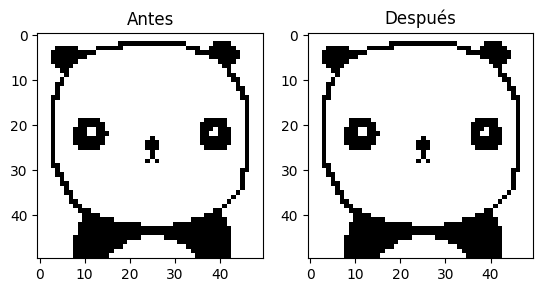
\includegraphics[width=0.8\linewidth]{imgs/ej1_1_1.png}}\\
    \subfloat[Imagen 2]{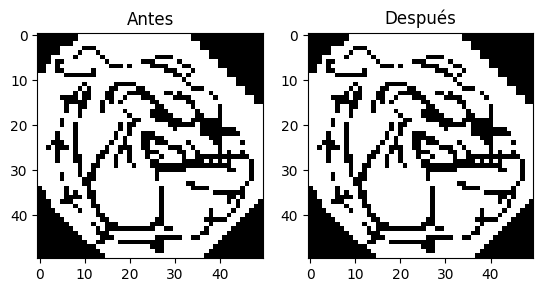
\includegraphics[width=0.8\linewidth]{imgs/ej1_1_2.png}}\\
    \subfloat[Imagen 3]{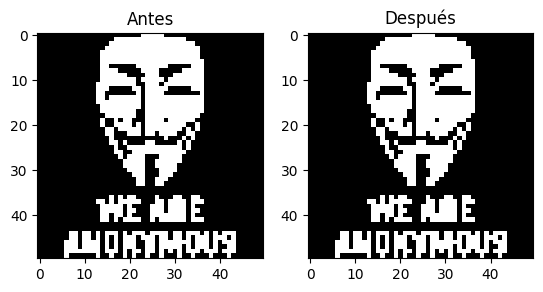
\includegraphics[width=0.8\linewidth]{imgs/ej1_1_3.png}}
    \caption{Imágenes del inciso 1 - Red 1.}
    \label{fig:ej1_a}
\end{figure}


\begin{figure}[p]
    \centering
    \subfloat[Imagen 4]{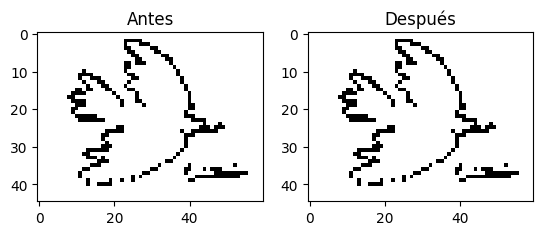
\includegraphics[width=0.8\linewidth]{imgs/ej1_1_4.png}}\\
    \subfloat[Imagen 5]{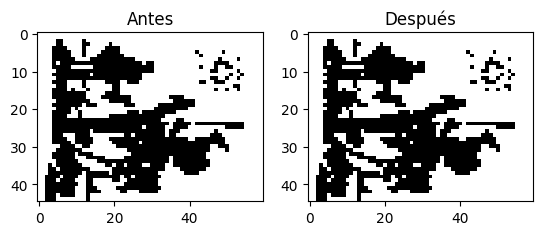
\includegraphics[width=0.8\linewidth]{imgs/ej1_1_5.png}}\\
    \subfloat[Imagen 6]{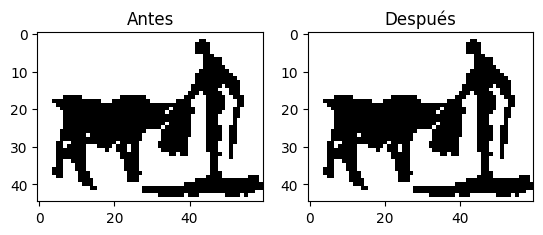
\includegraphics[width=0.8\linewidth]{imgs/ej1_1_6.png}}
    \caption{Imágenes del inciso 1 - Red 2.}
    \label{fig:ej1_b}
\end{figure}
\clearpage
\newpage

\clearpage
\begin{figure}[p]
    \centering
    \subfloat[Imagen 1]{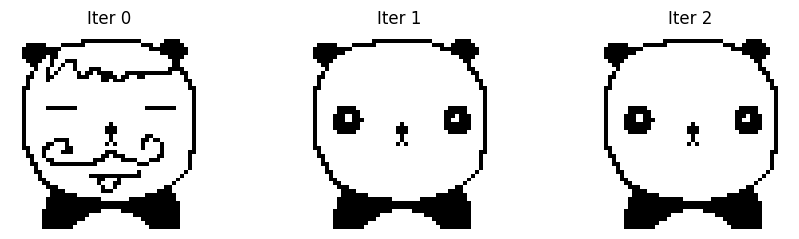
\includegraphics[width=1\linewidth]{imgs/ej1_2_1.png}}\\
    \subfloat[Imagen 2]{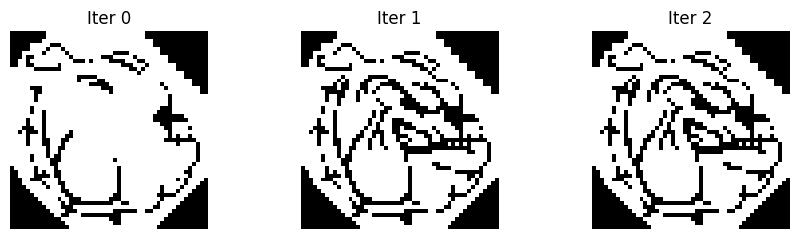
\includegraphics[width=1\linewidth]{imgs/ej1_2_2.png}}\\
    \subfloat[Imagen 3]{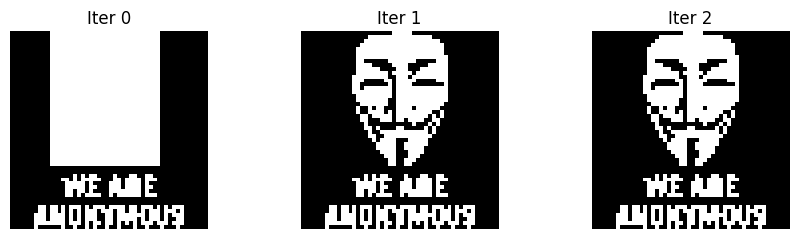
\includegraphics[width=1\linewidth]{imgs/ej1_2_3.png}}
    \caption{Imágenes del inciso 2 - Red 1.}
    \label{fig:ej2_a}
\end{figure}


\begin{figure}[p]
    \centering
    \subfloat[Imagen 4]{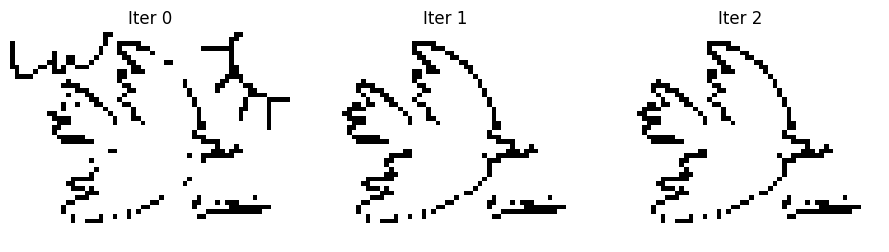
\includegraphics[width=1\linewidth]{imgs/ej1_2_4.png}}\\
    \subfloat[Imagen 5]{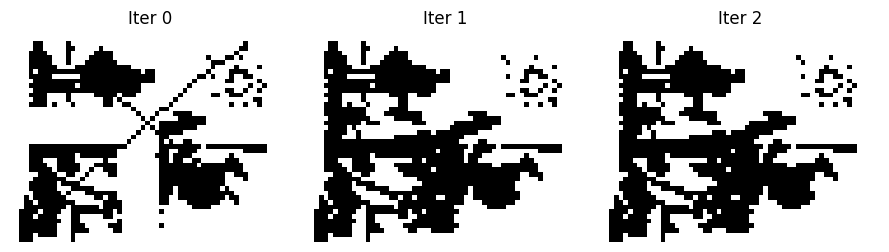
\includegraphics[width=1\linewidth]{imgs/ej1_2_5.png}}\\
    \subfloat[Imagen 6]{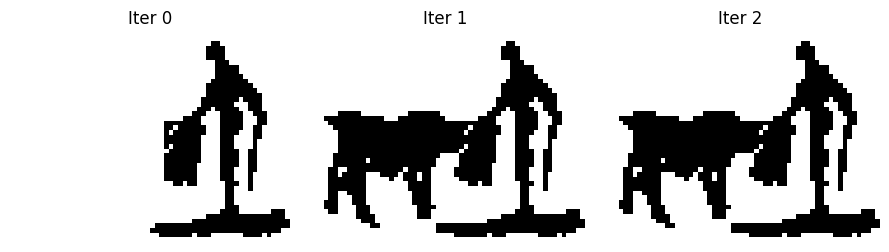
\includegraphics[width=1\linewidth]{imgs/ej1_2_6.png}}
    \caption{Imágenes del inciso 2 - Red 2.}
    \label{fig:ej2_b}
\end{figure}
\clearpage
\newpage

\begin{figure}[h!]
    \centering
    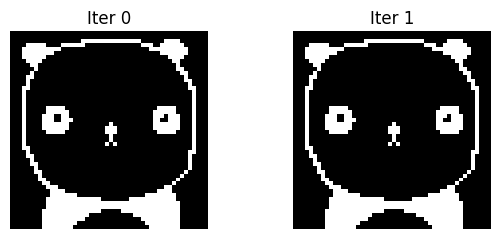
\includegraphics[width=0.8\linewidth]{imgs/ej1_3_1.png}
    \caption{El estado inverso del panda es estable.}
    \label{fig:ej1_3_1}
\end{figure}

\begin{figure}[h!]
    \centering
    
\includegraphics[width=0.8\linewidth]{imgs/ej1_3_2.png}
    \caption{El estado inverso del torero editado es un atractor.}
    \label{fig:ej1_3_2}
\end{figure}

\begin{figure}[h!]
    \centering
    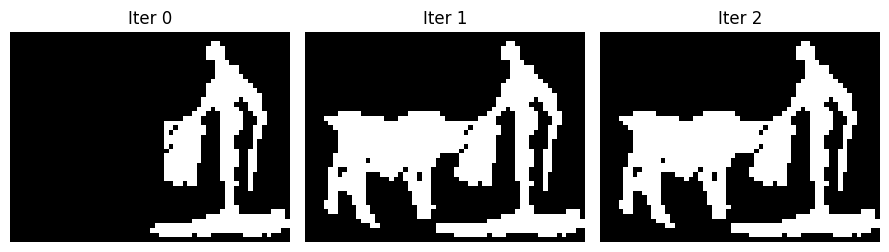
\includegraphics[width=1\linewidth]{imgs/ej1_3_3.png}
    \caption{La combinación lineal de los 3 estados enseñados a la red 1 es estable.}
    \label{fig:ej1_3_3}
\end{figure}

\begin{figure}[h!]
    \centering
    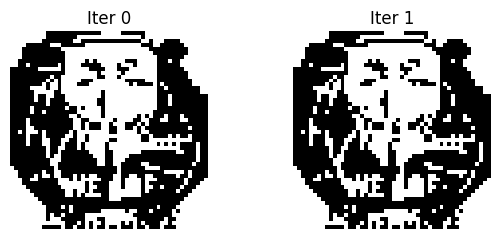
\includegraphics[width=0.8\linewidth]{imgs/ej1_3_4.png}
    \caption{La combinación lineal con un estado alterado es un atractor.}
    \label{fig:ej1_3_4}
\end{figure}

\begin{figure}[h!]
    \centering
    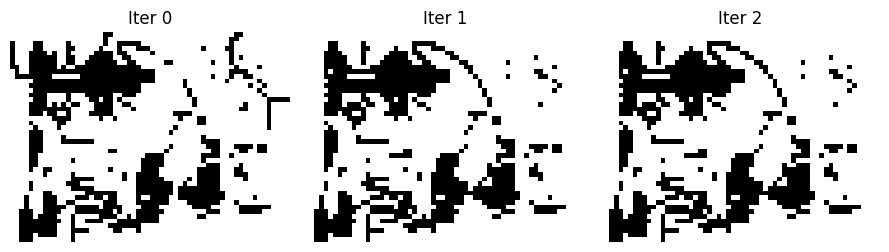
\includegraphics[width=1\linewidth]{imgs/ej1_3_5.png}
    \caption{La combinación lineal con un estado alterado es un atractor.}
    \label{fig:ej1_3_5}
\end{figure}
\clearpage
\newpage




\begin{figure}[h!]
    \centering
    % --- Primer fila: 2 columnas con 3 imágenes ---
    \begin{minipage}{0.48\linewidth}
        \centering
        \subfloat[]{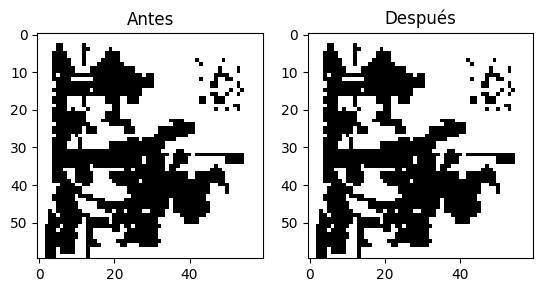
\includegraphics[width=\linewidth]{imgs/ej1_4_4.png}}\\
        \subfloat[]{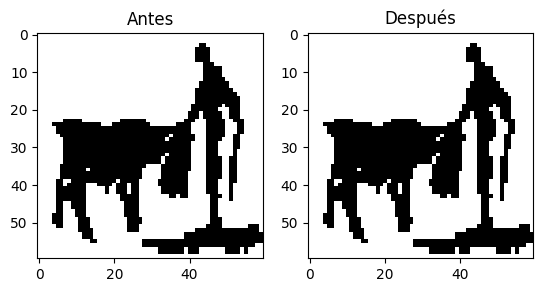
\includegraphics[width=\linewidth]{imgs/ej1_4_5.png}}\\
        \subfloat[]{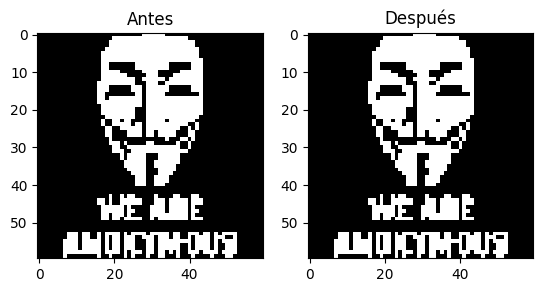
\includegraphics[width=\linewidth]{imgs/ej1_4_6.png}}
    \end{minipage}\hfill
    \begin{minipage}{0.48\linewidth}
        \centering
        \subfloat[]{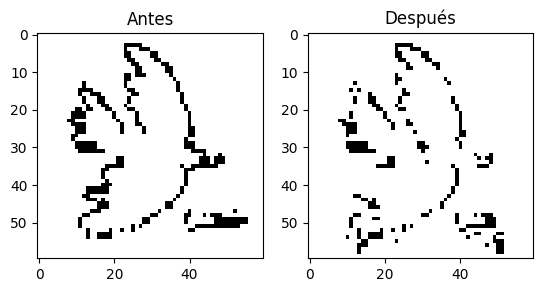
\includegraphics[width=\linewidth]{imgs/ej1_4_1.png}}\\
        \subfloat[]{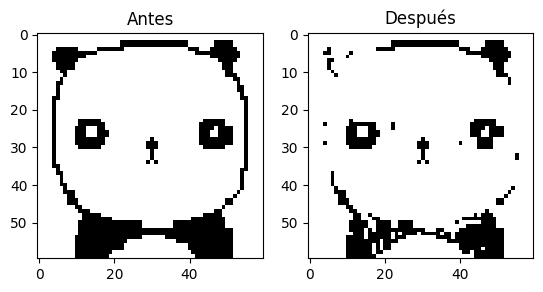
\includegraphics[width=\linewidth]{imgs/ej1_4_2.png}}\\
        \subfloat[]{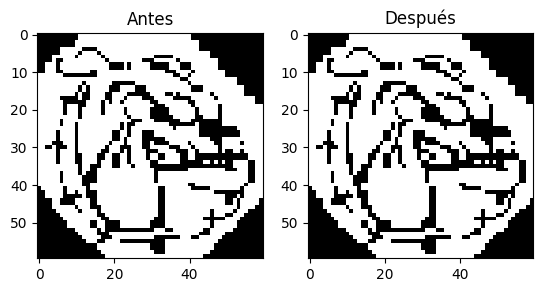
\includegraphics[width=\linewidth]{imgs/ej1_4_3.png}}
    \end{minipage}
\caption{\centering Imágenes enseñadas (a izquierda de cada subfigura) y recordadas (a derecha) con una red de $60 \times 60$}
    \label{fig:ej1_4}
\end{figure}


\begin{figure}[h!]
    \centering
    % --- Primer fila: 2 columnas con 3 imágenes ---
    \begin{minipage}{0.48\linewidth}
        \centering
        \subfloat[]{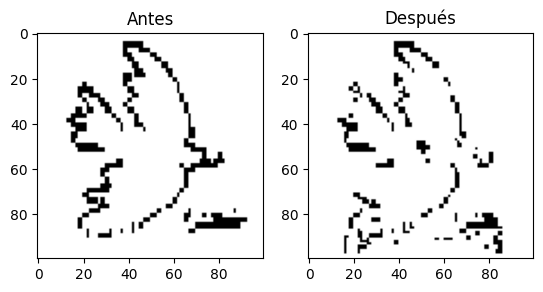
\includegraphics[width=\linewidth]{imgs/ej1_4_7.png}}\\
        \subfloat[]{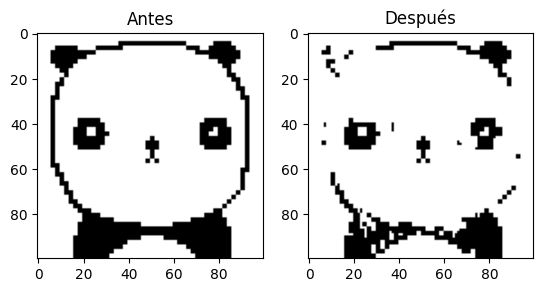
\includegraphics[width=\linewidth]{imgs/ej1_4_8.png}}\\
        \subfloat[]{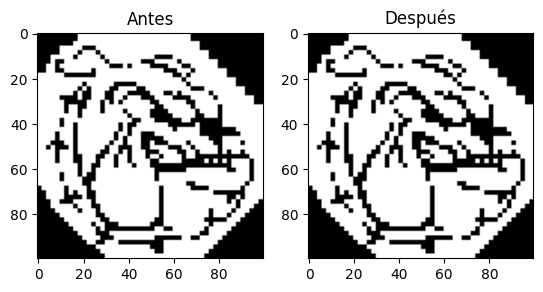
\includegraphics[width=\linewidth]{imgs/ej1_4_9.png}}
    \end{minipage}\hfill
    \begin{minipage}{0.48\linewidth}
        \centering
        \subfloat[]{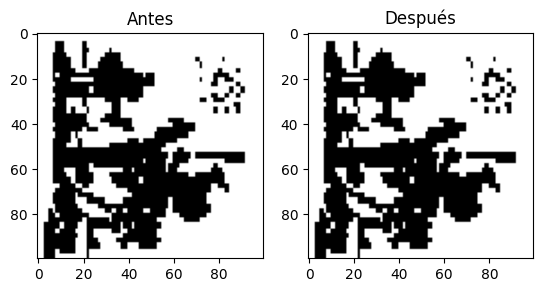
\includegraphics[width=\linewidth]{imgs/ej1_4_10.png}}\\
        \subfloat[]{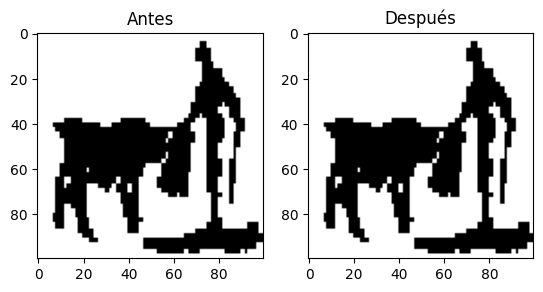
\includegraphics[width=\linewidth]{imgs/ej1_4_11.png}}\\
        \subfloat[]{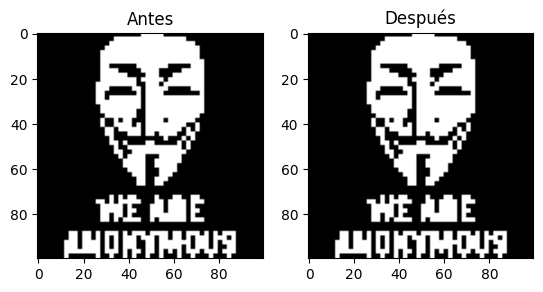
\includegraphics[width=\linewidth]{imgs/ej1_4_12.png}}
    \end{minipage}
\caption{\centering Imágenes enseñadas (a izquierda de cada subfigura) y recordadas (a derecha) con una red de $100 \times 100$}
    \label{fig:ej1_4_2}
\end{figure}

\clearpage
\newpage

\subsection{Análisis}

En los 4 incisos desarrollados no solo se ahondó en la implementación de una red de Hopfield con actualización sincrónica, sino que además se estudiaron la capacidad de memorización, una de sus limitaciones y la existencia de estados estables (atractores) en la red. 

El primer inciso evaluó la memoria de la red, verificando que los patrones enseñados fueran correctamente recordados. Ambas redes entrenadas lograron aprender los tres patrones  sin errores. Este resultado contrasta con lo observado en el inciso 4, donde no se pudieron memorizar todos los patrones. Esto sugiere que las limitaciones de una red neuronal no dependen únicamente de, por ejemplo, su cantidad de neuronas, sino también de las características de los datos: patrones demasiado similares entre sí reducen la capacidad efectiva de la red\footnote{siempre que la capacidad se mida con la expectativa de que el \textit{recall} sea perfecto, sin errores}.

Por otro lado, las redes no solo contienen los patrones enseñados, sino que también generan estados estables espurios. Estos atractores pueden atrapar a la red en configuraciones no deseadas, como la inversión de un patrón aprendido o una mezcla de varios.   Si el estado inicial $P$ es suficientemente cercano a uno de estos atractores, la red puede converger allí en lugar de al patrón buscado. Se considera que esto constituye una limitación no menor para aplicaciones prácticas en las que se espera que la red aprenda y recuerde un conjunto específico de patrones. 

Cabe destacar que, aún si no se probaron todos los estados espurios existentes, se considera que el objetivo académico de conocer de su existencia se cumplió. 

\clearpage
\newpage

\section{Ejercicio 2}

\subsection{Consignas}
\begin{enumerate}[label=\alph*]
\item Comprobar estadísticamente la capacidad de la red de Hopfield ‘82 calculando la
cantidad máxima de patrones pseudo-aleatorios aprendidos en función del tamaño
de la red. Obtener experimentalmente los resultados del cuadro~\ref{tab:1} (los
valores de la tabla corresponden a una iteración con actualización sincrónica).
\item Proponga una manera de generar patrones con distintos grados de correlación.
Utilice el método propuesto para analizar cómo varía la capacidad de la red de
Hopfield en función de la correlación entre patrones.
\end{enumerate}

\begin{table}[h!]
\centering
\begin{tabular}{|c|c|}
\hline
$P_{error}$ & $p_{max}/N$ \\ \hline
$0.001$     & $0.105$     \\ \hline
$0.0036$    & $0.138$     \\ \hline
$0.01$      & $0.185$     \\ \hline
$0.05$      & $0.37$      \\ \hline
$0.1$       & $0.61$      \\ \hline
\end{tabular}
\caption{Resultados teóricos de la capacidad de la red de Hopfield}
\label{tab:1}
\end{table}


\subsection{Desarrollo}

En este ejercicio se pide evaluar la capacidad de una red neuronal de Hopfield. En este contexto, la capacidad es función de la cantidad de neuronas y la probabilidad de error admisible, como se ve en las ecuaciones \eqref{eq:capacidad} y \eqref{eq:capacidad2}. 

\begin{equation}
\text{Capacidad}(P_{\text{error}} , N_{\text{neuronas}}) = \frac{\max N_{\text{patrones}} \quad \text{tq} \quad E_{tot}<P_{\text{error}}}{N_{\text{neuronas}}}
\label{eq:capacidad}
\end{equation}

\begin{equation}
E_{tot} = \frac{\text{\# neuronas equivocadas}}{N_{\text{neuronas}} \cdot N_{\text{patrones}}}
\label{eq:capacidad2}
\end{equation}

Los números provistos en el  cuadro~\ref{tab:1} se corresponden a una red de muchas neuronas entrenada con patrones descorrelacionados para varios umbrales de error, así que el primer experimento es entrenar una red de un tamaño adecuado (en este caso de 200 neuronas) y evaluar la capacidad en función de la probabilidad de cometer un error (un \textit{bit-flip}). La segunda parte del experimento consiste en ``barrer'' la correlación entre patrones para observar que sucede a medida que los patrones están más correlacionados. Como indica la bibliografía indicada en las consignas, esta capacidad usa solo una iteración para el cálculo de error, y existe la posibilidad de que pocos cambios causen una avalancha de cambios de estado, lo que implicaría que la capacidad es menor a la esperada. 

Para generar patrones correlacionados se parte de la definición de la correlación de Pearson y dos patrones generados aleatoriamente. Se suponen vectores X e Y generados de tal forma que toman valores discretos $-1$ y $1$ con probabilidad $1/2$. Así, sus medias son cero y las varianzas son unitarias. Se plantea el coeficiente de correlación de Pearson como:

\begin{equation}
corr_{coef} = \frac{\mathrm{cov}(X,Y)}{\sqrt{\mathrm{Var}(X)\cdot \mathrm{Var}(Y)}} =  E[X \cdot Y] - E[X]E[Y] = E[X \cdot Y]
\end{equation}

Ahora, $E[X \cdot Y]$ se puede expandir usando la esperanza total:

\begin{align*}
E[X \cdot Y] &= P(X=1)P(Y=1)\cdot (1\cdot 1) \\
&\quad + P(X=1)P(Y=-1)\cdot (1\cdot -1) \\
&\quad + P(X=-1)P(Y=1)\cdot (-1\cdot 1) \\
&\quad + P(X=-1)P(Y=-1)\cdot (-1\cdot -1)
\end{align*}

Denotando $p = P(X=Y)$ la probabilidad de que los vectores concuerden en algún bit, se obtiene:

\begin{equation}
E[X \cdot Y] = p - (1-p) = 2p-1
\end{equation}

Entonces:

\begin{equation}
corr_{coef} = 2p-1 \quad \Leftrightarrow \quad p = \frac{corr_{coef} +1}{2}
\end{equation}

De esta manera, se puede tomar un vector $X$ generado como cualquier vector aleatorio y luego generar un vector $Y$ en base a la probabilidad $p$ de que concuerde con $X$. Si $x=1$, se tira una ``moneda'' con probabilidad $p$ de que $y=x$.

En el código correspondiente a esta actividad se genera un primer vector y se guarda como ``semilla'' para generar el resto. 

\newpage
\subsubsection{Consigna a}

La idea general detrás del algoritmo implementado de calculo de capacidad de la red es simple: se crea una red de N neuronas y se itera desde 1 hasta N. En cada iteración se agrega un patrón más a la red (se actualiza la W) y se calcula cuantos errores tiene en la recuperación de todos los patrones contenidos en W. Luego, estos datos pueden usarse para estimar los intervalos de patrones enseñados que aseguren ciertas probabilidades de error. 

La figura \ref{fig:ej2_1_1} muestra la evolución de la capacidad de la red en función de la probabilidad de cometer un error para patrones con correlación de valor $0$ (coeficiente de correlación de Pearson). El cuadro~\ref{tab:2} muestra los datos en su forma tabular. La capacidad fue evaluada para los valores en el cuadro teórico. Se observa una coincidencia muy elevada entre los valores teóricos y los experimentales, con una diferencia relativa porcentual máxima de $2.7\%$. 


\begin{figure}[h!]
    \centering
    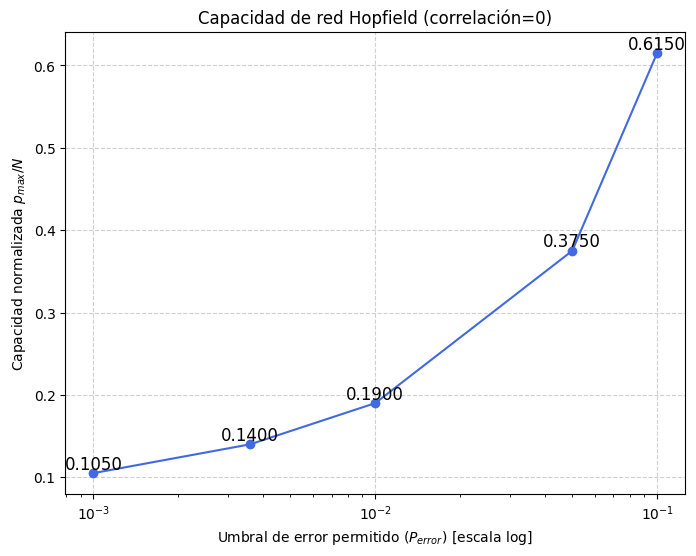
\includegraphics[width=0.8\linewidth]{imgs/ej2_1_1.png}
    \caption{Capacidad vs $P_{error}$. Correlación $= 0$}
    \label{fig:ej2_1_1}
\end{figure}

\begin{table}[h!]
\centering
\begin{tabular}{|c|c|c|}
\hline
$P_{error}$ & $p_{max}/N$ &Error relativo $\%$\\ \hline
$0.001$     & $0.105$ & 0   \\ \hline
$0.0036$    & $0.14$   &  1.45\\ \hline
$0.01$      & $0.19$   &  2.70\\ \hline
$0.05$      & $0.375$ &   1.35  \\ \hline
$0.1$       & $0.615$    & 0.82 \\ \hline
\end{tabular}
\caption{Resultados experimentales de la capacidad de la red de Hopfield}
\label{tab:2}
\end{table}

\newpage

\subsubsection{Consigna b}

El cuadro~\ref{tab:correlaciones} muestra como varía la capacidad en función de la correlación entre patrones y las probabilidades de error. Las figuras 13 a 18 muestran la evolución de la capacidad para cada correlación simulada. 

\begin{table}[h!]
\centering
\begin{tabular}{|c|c|c|c|c|c|c|}
\hline
$P_{error}$ & $p_{max}/N$ & $p_{max}/N$  & $p_{max}/N$ & $p_{max}/N$  &   $p_{max}/N$& $p_{max}/N$ \\ \hline
0.001  &   $0.025$    &    $0.015$   &   $0.01$    &    $0.01$   & $0.01$ &  $1$    \\ \hline
0.0036 &    $0.055$   &     $0.015$  &    $0.01$   &  $0.01$     &  $0.03$ &$1$     \\ \hline
0.01   &    $0.08$  &   $0.02$    &   $0.01$    &   $0.01$    &  $1$  &$1$    \\ \hline
0.05   &    $0.165$   &  $0.03$     &    $0.015$   &   $0.02$    &  $1$ &$1$     \\ \hline
0.1    &   $0.26$   &   $0.045$    &   $0.025$    &   $1$    &  $1$ &$1$     \\ \hline  \hline
Correlación  &0.2  &0.4&0.6&0.8&0.99&1 \\ \hline

\end{tabular}
\caption{Resultados experimentales de la capacidad de la red de Hopfield para distintas correlaciones}
\label{tab:correlaciones}
\end{table}

\begin{figure}[h!]
    \centering
    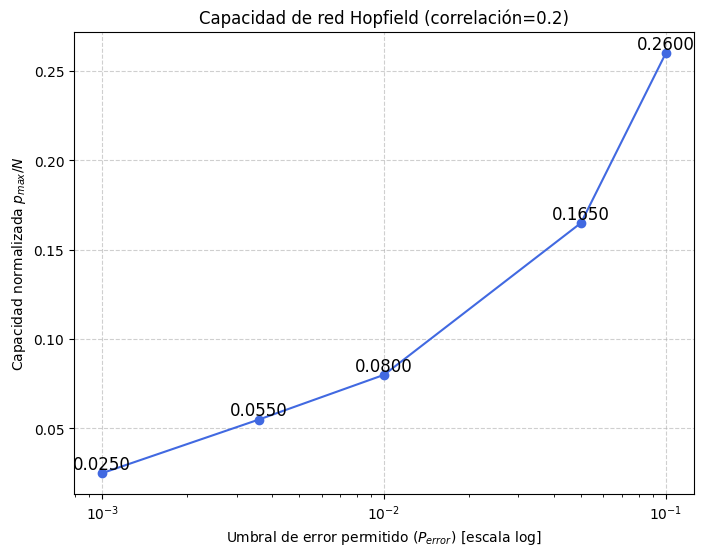
\includegraphics[width=0.8\linewidth]{imgs/ej2_2_1.png}
    \caption{Capacidad vs $P_{error}$. Correlación $= 0.2$}
    \label{fig:ej2_2_1}
\end{figure}

\begin{figure}[h!]
    \centering
    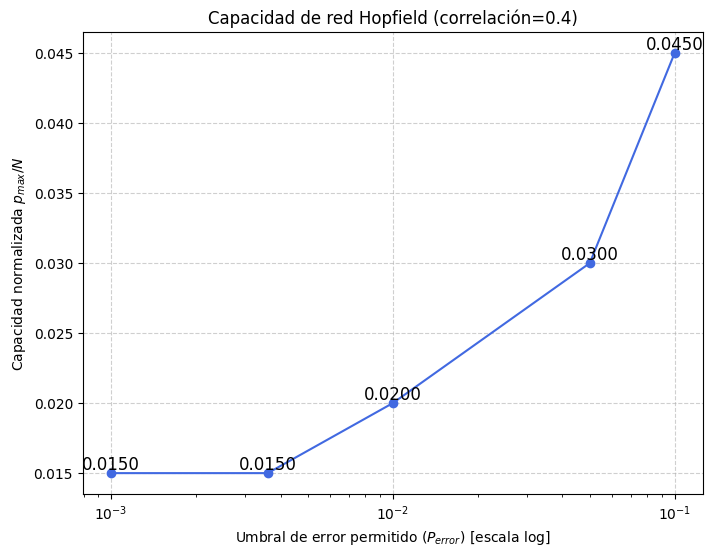
\includegraphics[width=0.8\linewidth]{imgs/ej2_2_2.png}
    \caption{Capacidad vs $P_{error}$. Correlación $= 0.4$}
    \label{fig:ej2_2_2}
\end{figure}

\begin{figure}[h!]
    \centering
    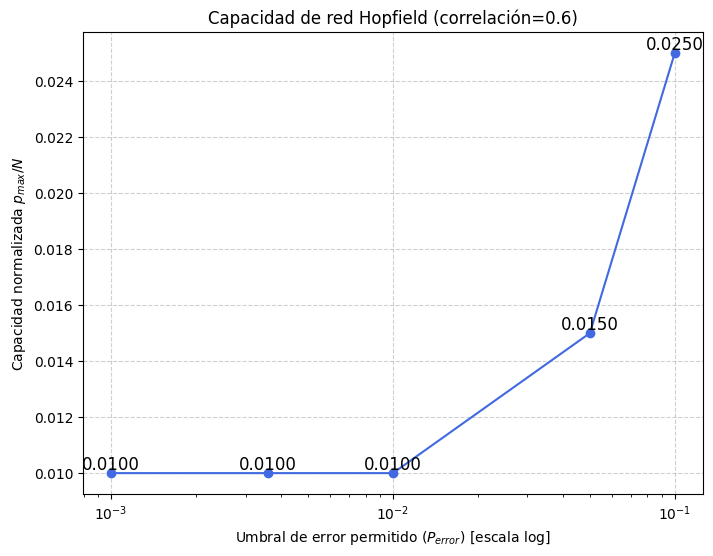
\includegraphics[width=0.8\linewidth]{imgs/ej2_2_3.png}
    \caption{Capacidad vs $P_{error}$. Correlación $= 0.6$}
    \label{fig:ej2_2_3}
\end{figure}

\begin{figure}[h!]
    \centering
    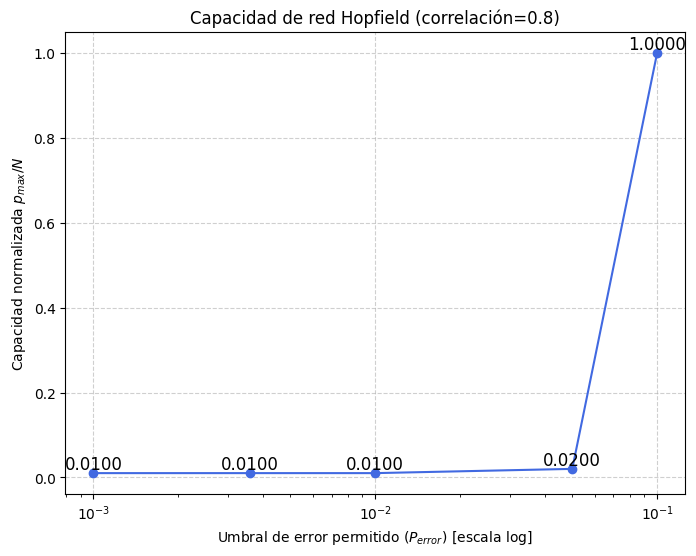
\includegraphics[width=0.8\linewidth]{imgs/ej2_2_4.png}
    \caption{Capacidad vs $P_{error}$. Correlación $= 0.8$}
    \label{fig:ej2_2_4}
\end{figure}

\begin{figure}[h!]
    \centering
    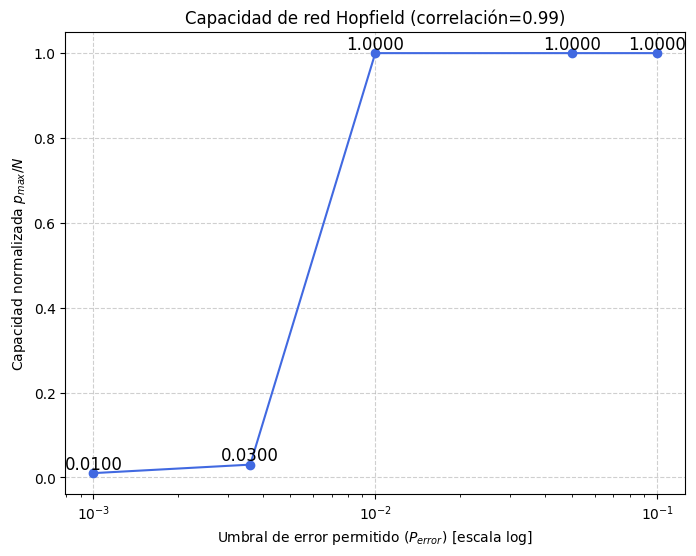
\includegraphics[width=0.8\linewidth]{imgs/corr099.png}
    \caption{Capacidad vs $P_{error}$. Correlación $= 0.99$}
    \label{img-0.99}
\end{figure}


\begin{figure}[h!]
    \centering
    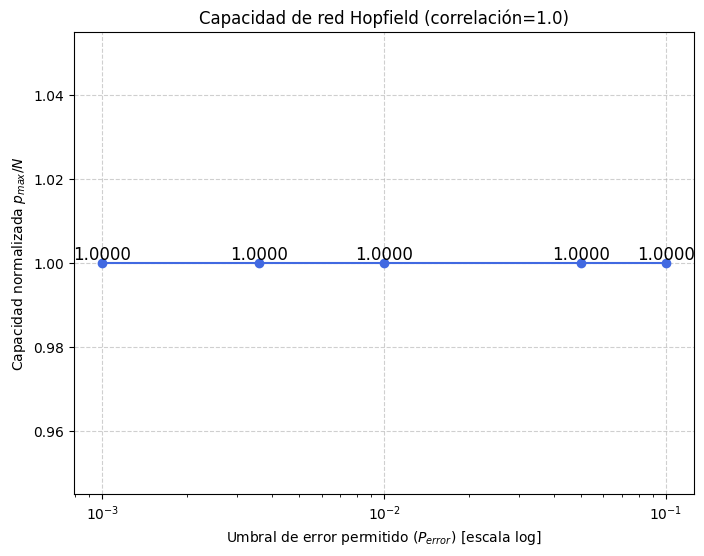
\includegraphics[width=0.8\linewidth]{imgs/ej2_2_5.png}
    \caption{Capacidad vs $P_{error}$. Correlación $= 1$}
    \label{fig:ej2_2_5}
\end{figure}

\clearpage
\newpage

\subsection{Análisis}

La capacidad teórica y la obtenida experimentalmente difieren por un error relativo máximo de $2.7 \%$, lo que indica una coincidencia prácticamente perfecta. Esta diferencia puede explicarse porque la capacidad teórica se calcula suponiendo una cantidad elevada (tendiente a infinito) de neuronas, mientras que en el experimento se utilizó una red de 200 neuronas. Además, los valores mostrados corresponden a un promedio de múltiples redes; aumentar el número de redes promedio podría acercar aún más los resultados al valor teórico.

Respecto a la capacidad en función de la correlación, se observa un comportamiento dual. Un incremento en la correlación causa una disminución en la capacidad para umbrales de error bajos debido a que la red termina aprendiendo una combinación de todos los estados enseñados, producto de la similitud entre patrones. Sin embargo, para umbrales de error altos, la similitud de los patrones y su cercanía al estado memorizado por la red causa un incremento en la capacidad. 

Este comportamiento sugiere una posible aplicación: Si se entrenara una red de este tipo con un conjunto de imágenes similares y luego se obtuviera el estado estable, la red podría utilizarse para identificar elementos pertenecientes a la misma categoría que los del set de entrenamiento. El funcionamiento sería análogo al de un clasificador basado en similitud de patrones pero de "si" o "no". Es decir, se puede entrenar una red para que aprenda el "arquetipo" de una clase (ej.: perros). Después del entrenamiento, si se le diera una imagen de un perro, la red convergería a un estado con cierta energía o "en cierto lugar", y lo que no es perro tal vez convergería a otra región, con otra energía. 

\section{Conclusiones}

A lo largo de este documento se implementaron varias redes de Hopfield con la finalidad de analizar varios aspectos de estas, como su memoria, capacidad, existencia de estados espurios y limitaciones. Se pudo denotar que el desempeño de una red neuronal no depende únicamente de la cantidad de neuronas, sino que también de los datos de entrenamiento (siempre teniendo en cuenta la finalidad de la red). Aparte, se demostró experimentalmente que la capacidad de una red neuronal de dicho tipo es la indicada en el cuadro~\ref{tab:1} con un error menor al $3\%$. Por último, se ahondó en la relación entre la capacidad, la correlación y la probabilidad de error, encontrando 2 tendencias marcadas de aumento y decremento de la capacidad. 



\end{document}
